\documentclass{article}

\begin{document}

\setlength{\parindent}{6ex}

\indent

In this section datasets and performance metrics will be explained. \par 
Datasets are used in the training and testing of detectors. Datasets consist of some 
specific types of objects, in object detection case they are images, and the 
corresponding ground-truth information about the categories in images that 
detector performs to detect. So, the mainly used datasets are Pascal Visual Object 
Classes (VOC) \cite{pascalvoc} and Microsoft COCO: Common Objects in Context 
\cite{mscoco}. \par

Pascal VOC datasets are formed based on two challenges: classification and detection. From the 
beginning year of 2005 to 2012, Pascal VOC challenges are developed. The number of classes and images 
is increased through challenges. The last challenge of Pascal VOC occurred in 2012. Dataset of 
2012 consists of 20 categories in 11.530 images. \par

MS COCO aims to present a dataset in which common objects are in their natural 
contexts. The data are taken from complex everyday scenes. COCO consists of 91 
object categories in 328k images. A comparison between Pascal VOC and MS COCO 
of instances per category is shown in figure \ref{fig:cocovspascal1}. \par

Another dataset we used to test analyzed detectors is the Multiple Object Tracking Benchmark 
(MOT) \cite{mot}. Although MOT is a dataset for tracking, in challenge MOT17Det, they provide a 
challenge for Pedestrian Detection. There are seven different video data provided for 
the training set with their ground-truth labels. We used this data as a test set. There are 
5316 frames to process with a total of 112297 pedestrians annotated. 

\begin{figure}
    \centering
    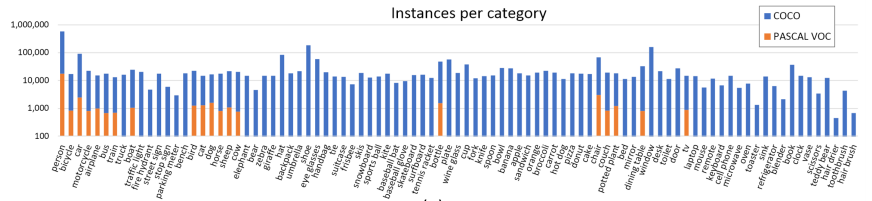
\includegraphics[width=\textwidth]{cocovspascal}
    \caption{Instances per category}
    \label{fig:cocovspascal1}
\end{figure}
\indent

Performance metrics are the way to measure the accuracy of detectors. In object 
detection, improving precision and recall yields to better test performance. The 
difference lies under the calculation of these metrics for object detection since 
correctly classifying the object in the image is not enough, the detector also correctly 
localizes the object in the image. So, to measure the correctness of each detection, 
a metric called Intersection over Union is used.

\begin{figure}
    \centering
    
\includegraphics[width=\textwidth]{iou}
    \caption{A visualization of IoU}
    \label{fig:iou1}
\end{figure}

\begin{table}[]
    \centering
    \begin{tabular}{|c|c|c|c|}
    \hline
    \multicolumn{2}{|c|}{\multirow{2}{*}{}}                                               & \multicolumn{2}{c|}{Ground-truth Value}                                         \\ \cline{3-4} 
    \multicolumn{2}{|c|}{}                                                                & Positive       & Negative                                                 \\ \hline
    \multirow{2}{*}{\begin{tabular}[c]{@{}c@{}}Predicted\\ Value\end{tabular}} & Positive & True Positive  & \begin{tabular}[c]{@{}c@{}}False\\ Positive\end{tabular} \\ \cline{2-4} 
                                                                               & Negative & False Negative & \begin{tabular}[c]{@{}c@{}}True\\ Negative\end{tabular}  \\ \hline
    \end{tabular}
    \caption{Table to understand concepts of classification of a prediction}
    \label{table:1}
\end{table}

\begin{itemize}
    \item Intersection over Union (IoU)
    IoU is the ratio between the intersection of predicted and ground-truth bounding box 
    divided by the union of predicted and ground-truth bounding box. The figure \ref{fig:iou1} is a 
    visualization of IoU to help to have a better intuition.
    \item Correctness of Detection
    IoU is used as a threshold to identify a detection as positive or negative. The 
    most commonly used IoU threshold is 0.5 which means if IoU value of a detection is 
    bigger than 0.5, that detection is counted as True Positive; otherwise, False Positive.
    \item The following concepts are used by the metrics:
    \begin{itemize}
        \item Ground-truth (GT): The true annotations on a given frame.
        \item True Positive (TP): A correct detection, IoU $\geq$ threshold. 
        \item False Positive (FP): A wrong detection, IoU $\leq$ threshold.
        \item False Negative (FN): A ground-truth not detected.
        \item True Negative (TN): Since many possible bounding boxes do not contain any object, 
        counting corrected misdetection is not necessarily needed.
        \item A better intuition can be obtained by looking into table \ref{table:1}.
    \end{itemize}
    \item These calculated concepts above are used to measure two main metrics: precision and 
    recall. Precision is the ratio of true positives to the sum of true positives and false 
    positives which provides the ratio of how accurate are your predictions. The recall is the ratio 
    of true positives to the sum of true positives and false negatives which indicates the ratio of 
    finding positives in all positives.
    \item The performance indicator for detectors is mean average precision. The average precision of a 
    category can be calculated by calculating the area under the precision-recall curve. Then, the mean 
    average precision is calculated by calculating average precision for all categories and divide 
    this total AP by the number of categories. In Pascal VOC, AP is calculated by using interpolation. 
    The 11-point interpolated precision-recall curve is used. Corresponding precision values of 11 recall 
    points are summed up and this value is divided by 11. Another way is to calculate all area under 
    the precision-recall curve which is used in later year competitions of Pascal VOC. In MS COCO, 
    101-point interpolated AP calculation is used. In MOT17Det, 11-point interpolated AP is used.
    \item False Alarm Rate (FAR) is calculated per frame. A false alarm is equivalent to a false positive. 
    Detector assumes an object is present in some location, although there is no object in that same position. 
    So, False Alarm Rate per frame is calculated by dividing the number of false positives to the number of 
    frames in the dataset. The relation of FAR and FP can be observed in table \ref{table:3}.
    \item Multiple Object Detection Accuracy (MODA) is calculated by using weighted-sum of FN and 
    FP per frame and this sum is divided by the number of ground-truth objects in that frame. So, the 
    higher the MODA value corresponds to a better performance in a detector.
    \item Multiple Object Detection Precision (MOTP) is calculated by using the overlap between ground-truth 
    and predicted object. In other terms, for a given frame, all objects' IoU values are calculated with 
    corresponding to their ground-truth boxes and these values are summed up. Then, this sum is divided by 
    the number of total ground-truth boxes in that frame. Thus, the higher MOTP value corresponds to a better 
    performance in a detector. 
\end{itemize}


\begin{figure}
    \begin{subfigure}{0.30\textwidth}%
        \centering
        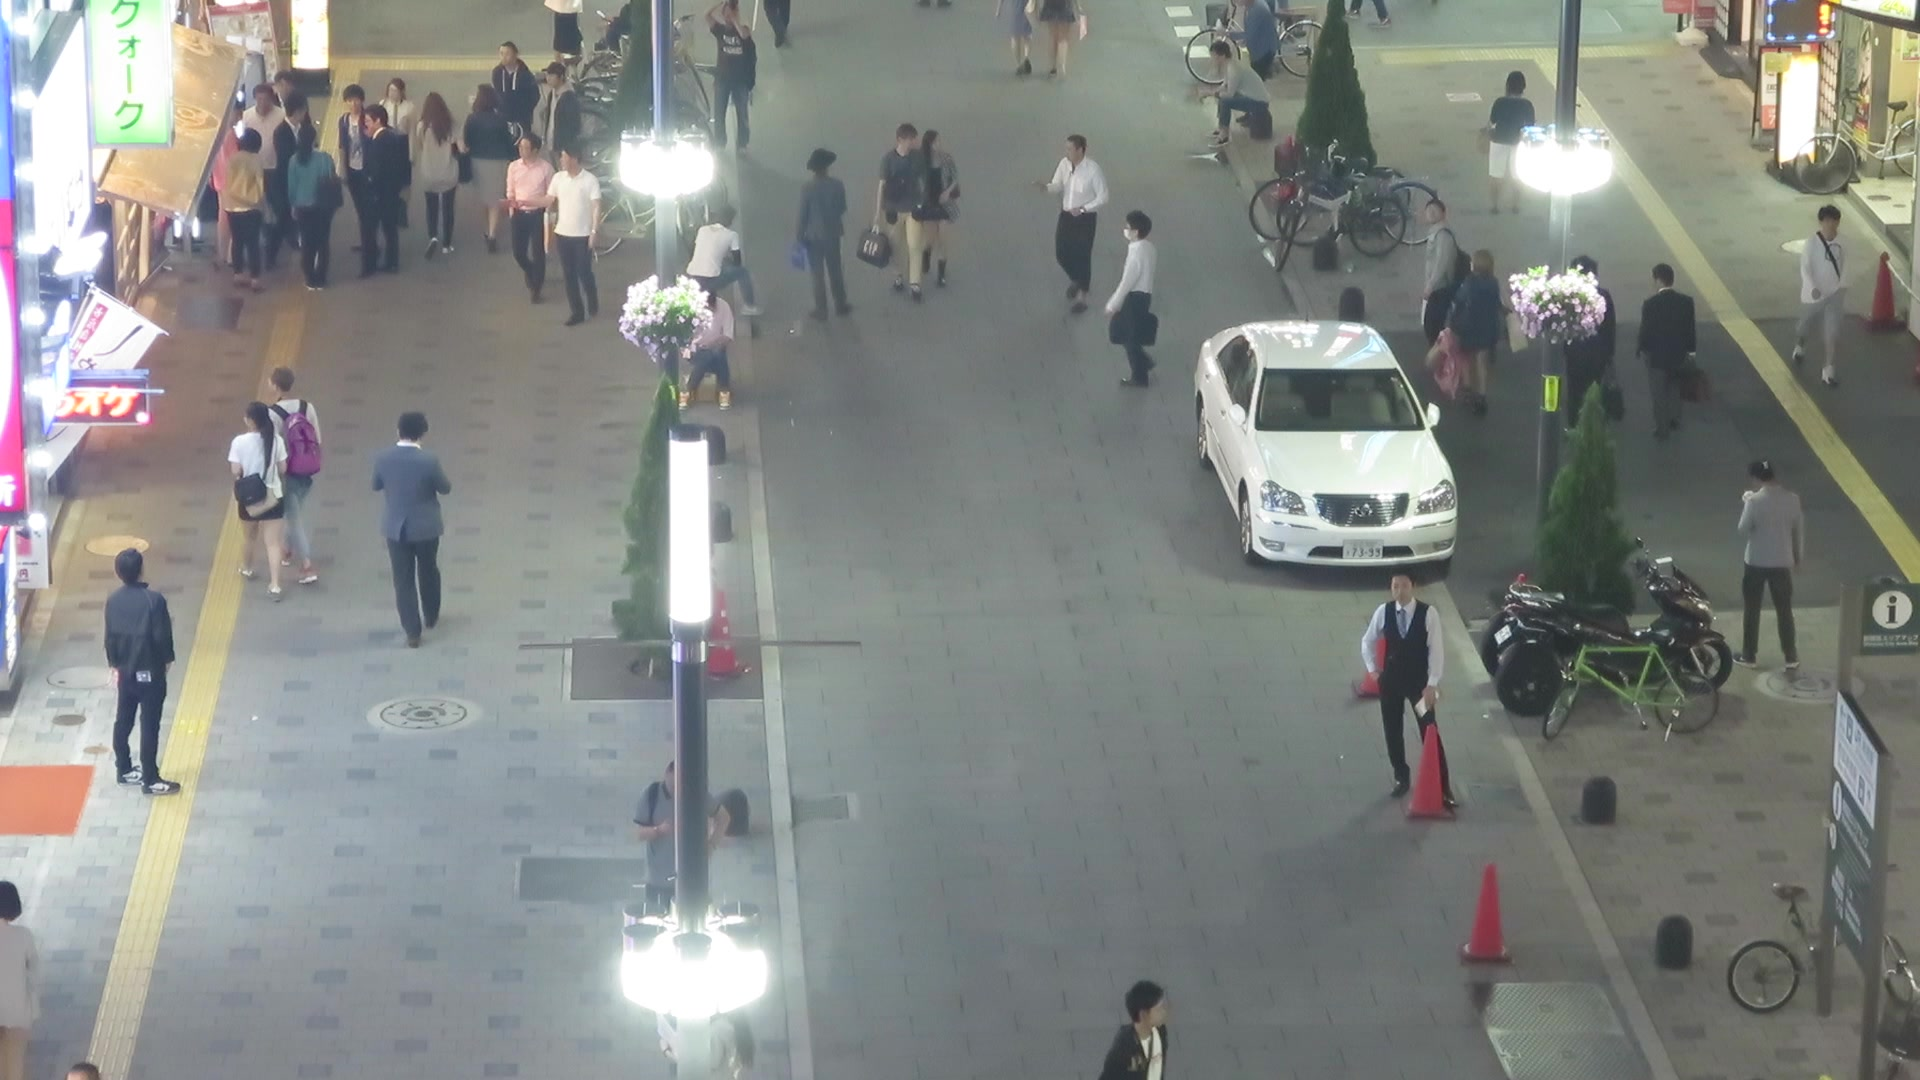
\includegraphics[width=\linewidth]{th_detection/org_img.png}
        \caption{Original Image}
        \label{fig:sfig1}
    \end{subfigure}     
    \begin{subfigure}{0.30\textwidth}%
        \centering
        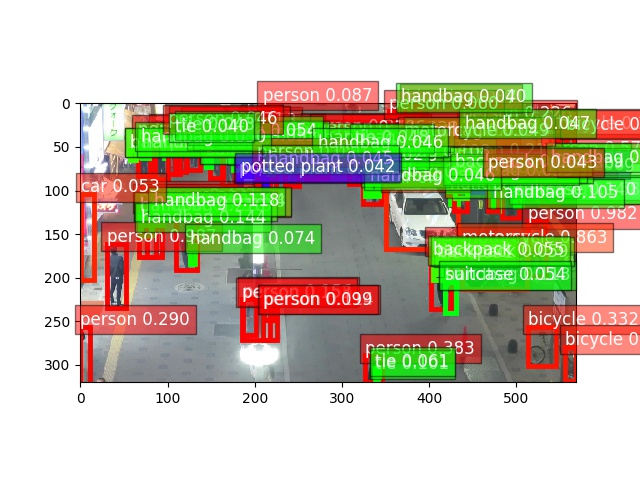
\includegraphics[width=\linewidth]{th_detection/0_0_th.png}
        \caption{No threshold}
        \label{fig:sfig2}
    \end{subfigure}
    \begin{subfigure}{0.30\textwidth}%
        \centering
        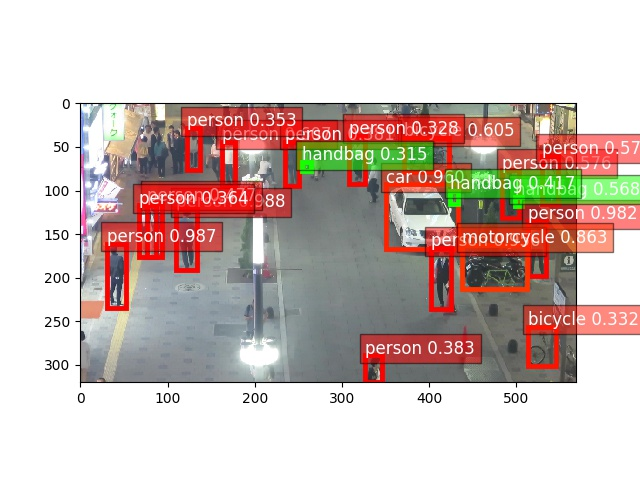
\includegraphics[width=\linewidth]{th_detection/0_3_th.png}
        \caption{0.3 threshold}
        \label{fig:sfig3}
    \end{subfigure}


    
    \begin{subfigure}{0.30\textwidth}%
        \centering
        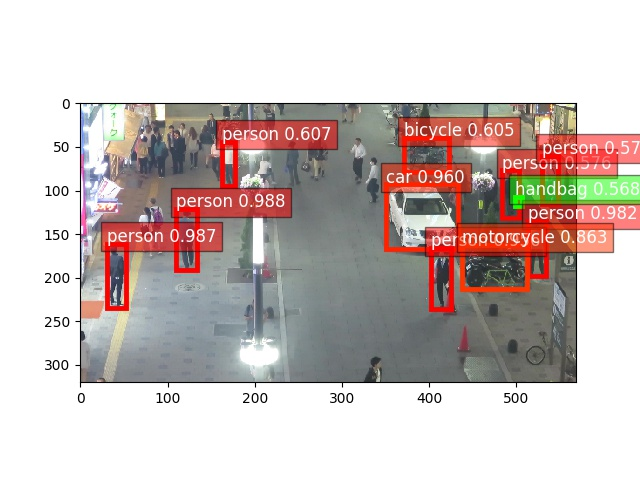
\includegraphics[width=\linewidth]{th_detection/0_5_th.png}
        \caption{0.5 threshold}
        \label{fig:sfig4}
    \end{subfigure}
    \begin{subfigure}{0.30\textwidth}%
        \centering
        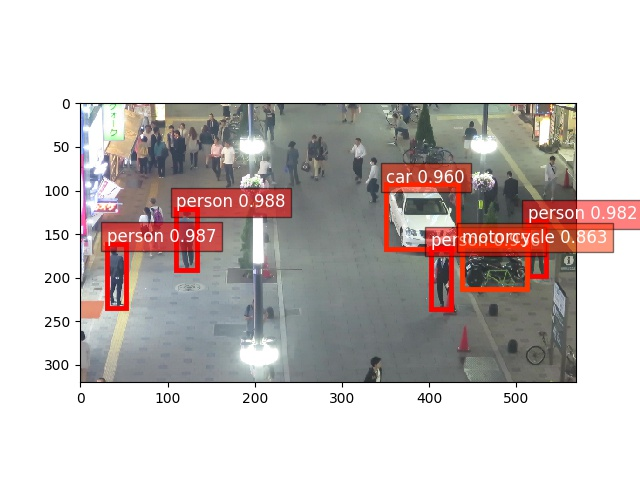
\includegraphics[width=\linewidth]{th_detection/0_7_th.png}
        \caption{0.7 threshold}
        \label{fig:sfig5}
    \end{subfigure}
    \begin{subfigure}{0.30\textwidth}%
        \centering
        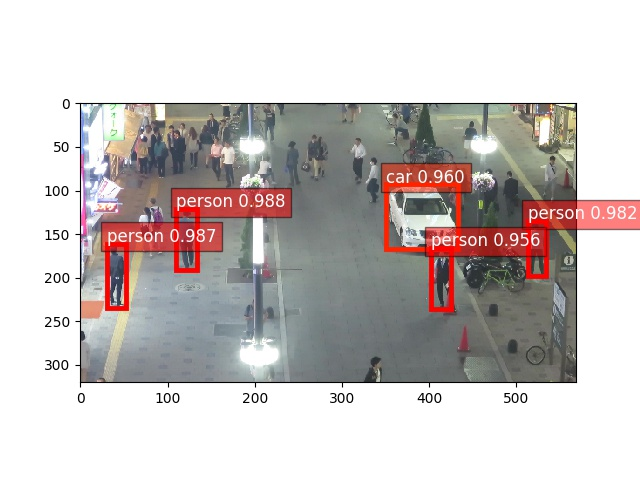
\includegraphics[width=\linewidth]{th_detection/0_9_th.png}
        \caption{0.9 threshold}
        \label{fig:sfig6}
    \end{subfigure}
    \caption{Examples of detected boxes for different thresholds in YOLOv3 320x320}
    \label{fig:exp_imgs}
\end{figure}


\end{document}